\documentclass{beamer}
\usepackage{ragged2e} % \justifying
\usepackage{bm}
\usepackage{tensor}
\usetheme{metropolis}           % Use metropolis theme
\title{FP2: Torso Pose Estimation on the \\HRP4 Humanoid Robot}
\subtitle{Michele Cipriano, Godwin K. Peprah, Lorenzo Vianello}
\date{}
\author{\textit{Supervisor:} Nicola Scianca\\
    \textit{Professors:} Giuseppe Oriolo, Alessandro De Luca\\}
\institute{Autonomous and Mobile Robotics, Robotics 2\\
    Department of Computer, Control and Management
    Engineering\\Sapienza University of Rome}

% Fontsize of figure smaller than normalsize:
\setbeamerfont{caption}{size=\scriptsize}

\begin{document}
\nocite{*}

    \maketitle

    \begin{frame}{Introduction}
        Intro.
    \end{frame}

    \begin{frame}{Kinematic Model}
        Todo.
    \end{frame}

    \begin{frame}{Extended Kalman Filter}
        Todo.
    \end{frame}

    \begin{frame}{Accelerometer Integration}
        Todo.
    \end{frame}

    \begin{frame}{Gyroscope Integration}
        Todo.
    \end{frame}

    \begin{frame}{IMU}
        Experiments (5.1).
    \end{frame}

    \begin{frame}{Filtering Linear Velocities}
        Todo.
    \end{frame}

    \begin{frame}{Trilateration}
        Todo.
    \end{frame}

    \begin{frame}{MPC Loop Closure}
        Todo.
    \end{frame}

    \section{Regulation}

    \begin{frame}{Kinematic Model of the Unicycle}
        Brief description:
        \begin{align*}
            \dot{x} &= v \text{cos}(\theta) \\
            \dot{y} &= v \text{sin}(\theta) \\
            \dot{\theta} &= \omega
        \end{align*}
        with $v$ and $\omega$ respectively linear and angular velocity.
    \end{frame}

    \begin{frame}{Proportional Controller}
        \justifying
        Control law:
        \begin{align*}
            v &= k_1 \left\| \bm{p}_g - \bm{\hat{p}}_t \right\| \\
            \omega &= k_2 e_{\theta}
        \end{align*}
        with $e_\theta$ angle between the sagittal vector of the unicycle
        and the vector pointing from the unicycle towards the goal, $k_1 =
        0.18$ and $k_2 = 0.014$. Forcing $v$ and $\omega$ to zero when
        $\left\|\bm{p}_g - \bm{\hat{p}}_t \right\| < 0.25$.
        Desired and final configuration:
        \begin{align*}
            \bm{q}_g &= (-3, 5, \cdot)^T \\
            \bm{q}_f &= (-2.798, 5.090, 0.98\pi)^T \\
            \bm{\hat{q}}_f &= (-2.885, 5.127, 0.979\pi)^T
        \end{align*}
    \end{frame}

    %\begin{frame}{Proportional Controller}
    %    Desired and final configuration:
    %    \begin{align*}
    %        \bm{q}_g &= (-3, 5, \cdot)^T \\
    %        \bm{q}_f &= (-2.798, 5.090, 0.98\pi)^T \\
    %        \bm{\hat{q}}_f &= (-2.885, 5.127, 0.979\pi)^T
    %    \end{align*}
    %\end{frame}

    \begin{frame}{Proportional Controller: x-y Plot}
        \begin{figure}
            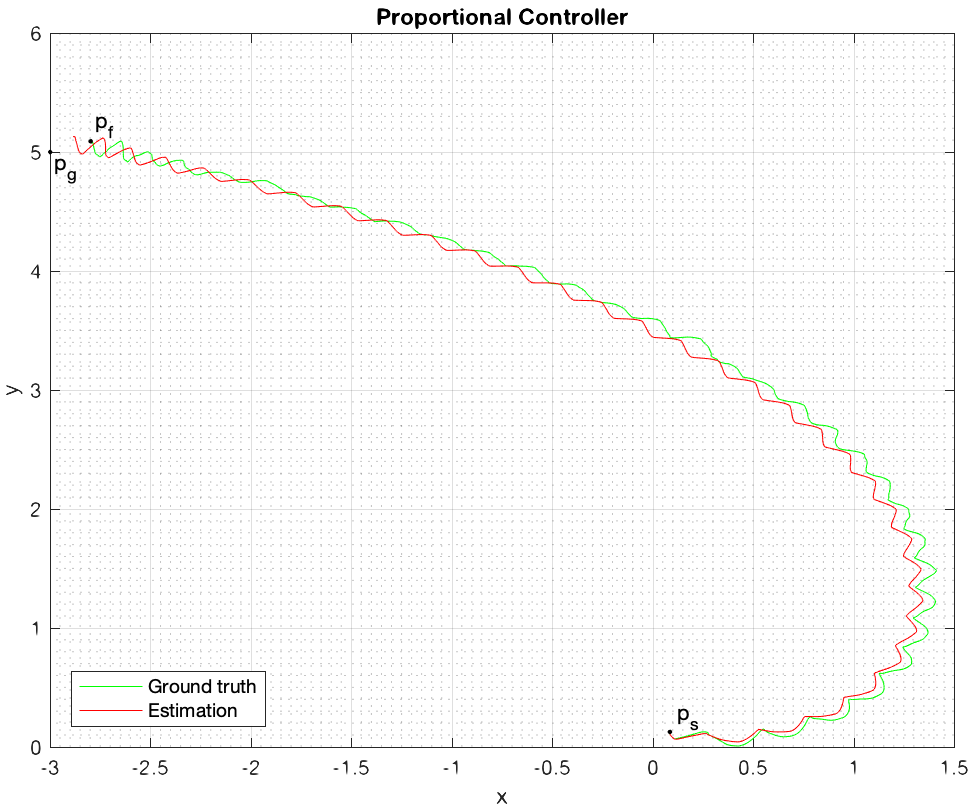
\includegraphics[width=0.85\textwidth]{images/proportional_controller.png}
        \end{figure}
    \end{frame}

    \begin{frame}{Cartesian Regulation}
        \justifying
        Let's express the coordinates of the unicycle in a reference frame
        $\mathcal{F}_g$ fixed at a position $(x_g, y_g)^T$ and
        rotated by $\theta_g$ around $\mathcal{F}_w$:
        \begin{equation*}
            \begin{pmatrix}
                \tensor[^g]{x}{} \\
                \tensor[^g]{y}{} \\
                \tensor[^g]{\theta}{}
            \end{pmatrix}
                =
            \bm{R}_z^T(\theta_g)
            \begin{pmatrix}
                x - x_g \\
                y - y_g \\
                \theta - \theta_g
            \end{pmatrix}
        \end{equation*}
    \end{frame}

    \begin{frame}{Cartesian Regulation}
        \justifying
        Control law:
        \begin{align*}
            v &= -k_1 (\tensor[^g]{x}{} \text{cos}(\tensor[^g]{\theta}{}) + \tensor[^g]{y}{} \text{sin}(\tensor[^g]{\theta}{})) \\
            \omega &=  k_2 (\text{Atan2}(\tensor[^g]{y}{}, \tensor[^g]{x}{}) - \tensor[^g]{\theta}{} + \pi)
        \end{align*}
        with $k_1 = 0.07$ and $k_2 = 0.01$. Forcing $v$ and $\omega$ to zero when
        $\left\|\bm{p}_g - \bm{\hat{p}}_t \right\| < 0.2$.
        Desired and final configuration:
        \begin{align*}
            \bm{q}_g &= (-2, 3.2, \cdot)^T \\
            \bm{q}_f &= (-1.788, 3.105, 1.562\pi)^T \\
            \bm{\hat{q}}_f &= (-1.823, 3.108, 1.562\pi)^T
        \end{align*}
    \end{frame}

    \begin{frame}{Cartesian Regulation: x-y Plot}
        \begin{figure}
            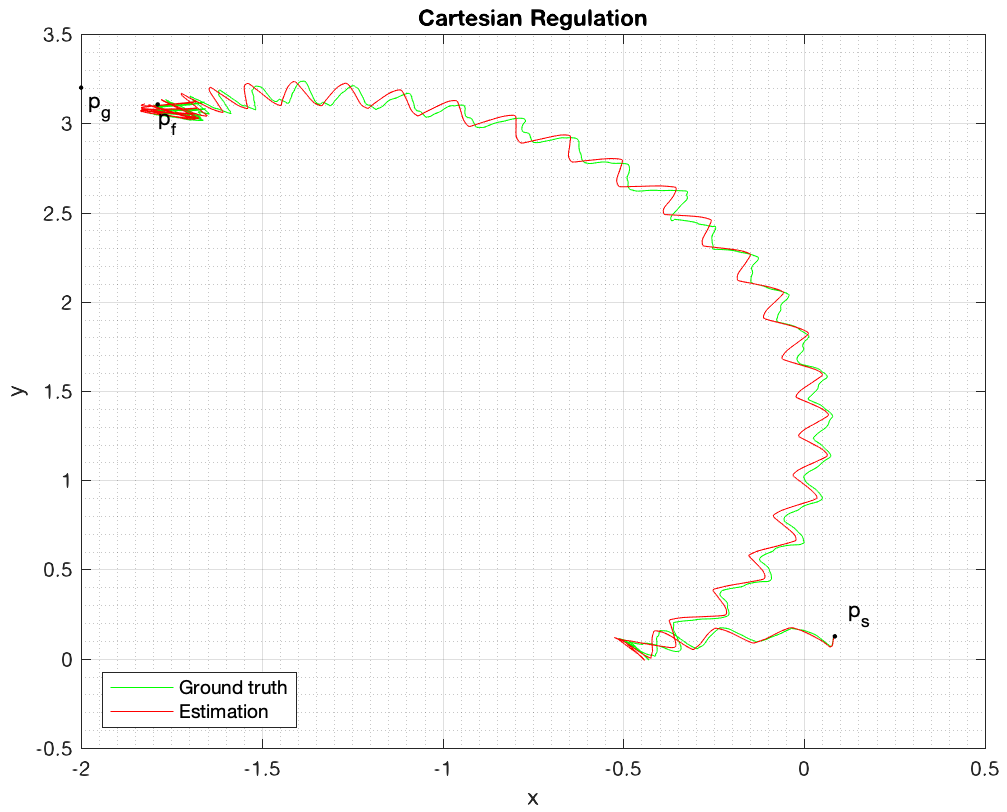
\includegraphics[width=0.85\textwidth]{images/cartesian_regulation.png}
        \end{figure}
    \end{frame}

    \begin{frame}{Kinematic Model of the Unicycle in Polar Coordinates}
        \justifying
        Brief description:
        \begin{align*}
            \dot{\rho}_r &= -v \text{cos}(\gamma_r) \\
            \dot{\gamma}_r &= \frac{\text{sin}(\gamma_r)}{\rho_r}v - \omega \\
            \dot{\delta}_r &= \frac{\text{sin}(\gamma_r)}{\rho_r}v
        \end{align*}
        Polar coordinates can be obtained from the generalized
        coordinates of the unicycle $(x, y, \theta)^T$ by computing:
        \begin{align*}
            \rho_r &= \sqrt{\tensor[^g]{x}{^2} + \tensor[^g]{y}{^2}} \\
            \gamma_r &= \text{Atan2}(\tensor[^g]{y}{}, \tensor[^g]{x}{}) - \tensor[^g]{\theta}{} + \pi \\
            \delta_r &= \gamma_r + \tensor[^g]{\theta}{}
        \end{align*}
    \end{frame}

    \begin{frame}{Posture Regulation}
        \justifying
        Control law:
        \begin{align*}
            v &= k_1 \rho_r \text{cos}(\gamma_r) \\
            w &= k_2 \gamma_r + k_1 \frac{\text{sin}(\gamma_r) \text{cos}(\gamma_r)}{\gamma_r}(\gamma_r + k_3 \delta_r)
        \end{align*}
        with $k_1 = 0.1$, $k_2 = 0.007$ $k_3 = 0.004$. Forcing $v$ and $\omega$ to zero when
        $\rho_r < 0.2$. Desired and final configuration:
        \begin{align*}
            \bm{q}_g &= (-2, 3.2, \pi)^T \\
            \bm{q}_f &= (-1.797, 3.194, 1.024\pi)^T \\
            \bm{\hat{q}}_f &= (-1.824, 3.222, 1.024\pi)^T \\
            \bm{\bar{q}}_f &= (-1.282, 3.424, 0.912\pi)^T
        \end{align*}
    \end{frame}

    \begin{frame}{Posture Regulation: x-y Plot}
        \begin{figure}
            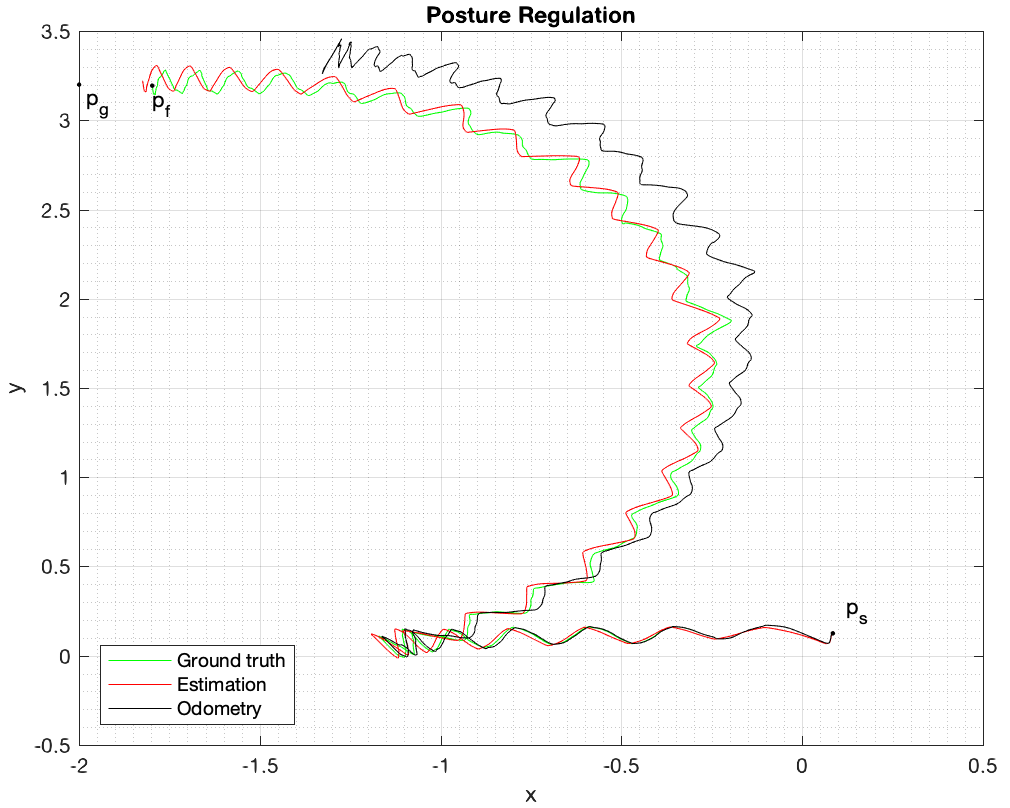
\includegraphics[width=0.85\textwidth]{images/posture_regulation.png}
        \end{figure}
    \end{frame}

    \begin{frame}{Posture Regulation: Yaw Plot}
        \begin{figure}
            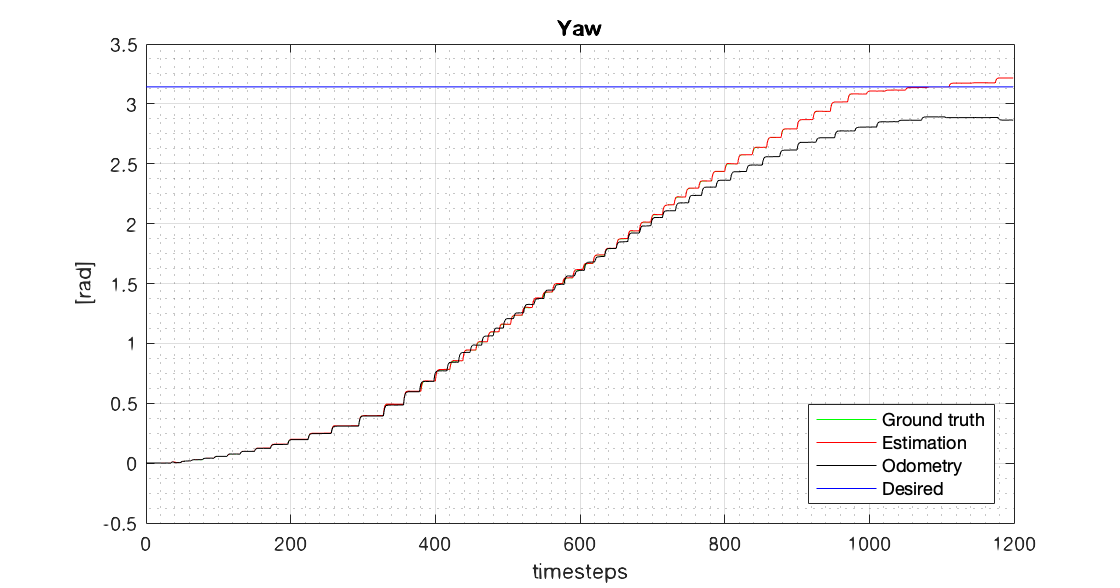
\includegraphics[width=\textwidth]{images/yaw_postureregulation.png}
        \end{figure}
    \end{frame}

    \begin{frame}{Posture Regulation: Velocity Profile Plots}
        \begin{figure}
            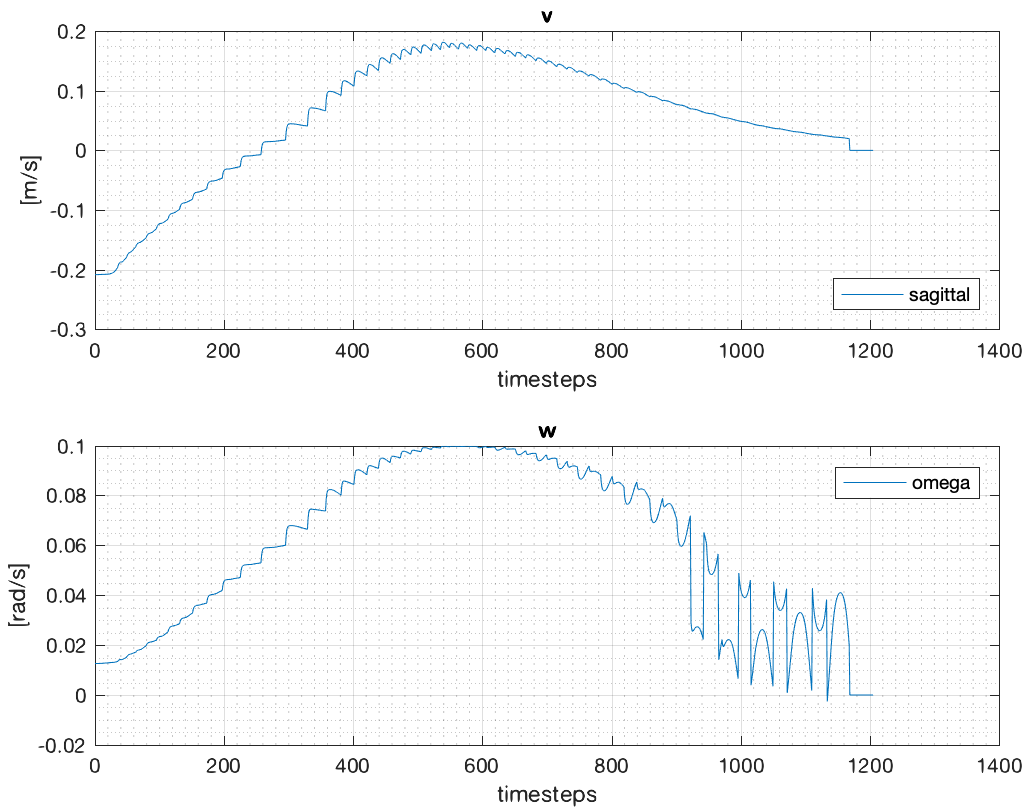
\includegraphics[width=0.9\textwidth]{images/unicycle_velocities.png}
        \end{figure}
    \end{frame}

    \begin{frame}{Conclusion}
        Conclusion.
    \end{frame}

    \begin{frame}[standout]
        Q\&A
    \end{frame}

    \appendix

    \begin{frame}{References}
        \bibliography{bibliography}
        \bibliographystyle{ieeetr}
    \end{frame}

\end{document}
